\documentclass[12pt,a4paper]{report}
\usepackage[latin1]{inputenc}
\usepackage{amsmath}
\usepackage{amsfonts}
\usepackage{amssymb}
\usepackage{graphicx}
\usepackage[left=2cm,right=2cm,top=2cm,bottom=2cm]{geometry}
\title{{\normalsize M.Sc. Simulation Sciences, Winter Semester 2012/2013}\\Fast Iterative Solvers\\{\normalsize Project 1: GMRES and CG}}			
\author{{\normalsize Group Members: \\{\small Abhishek Y. Deshmukh, R. Varun Raj, Raghavan Lakshmanan, Mohsin Ali Chaudry}}}	
\date{{\small June 10, 2013}}
\renewcommand*\thesection{\arabic{section}}
\begin{document}
\maketitle
\section{Plots: Error and Residual Vs. Iteration Index}
\begin{center}
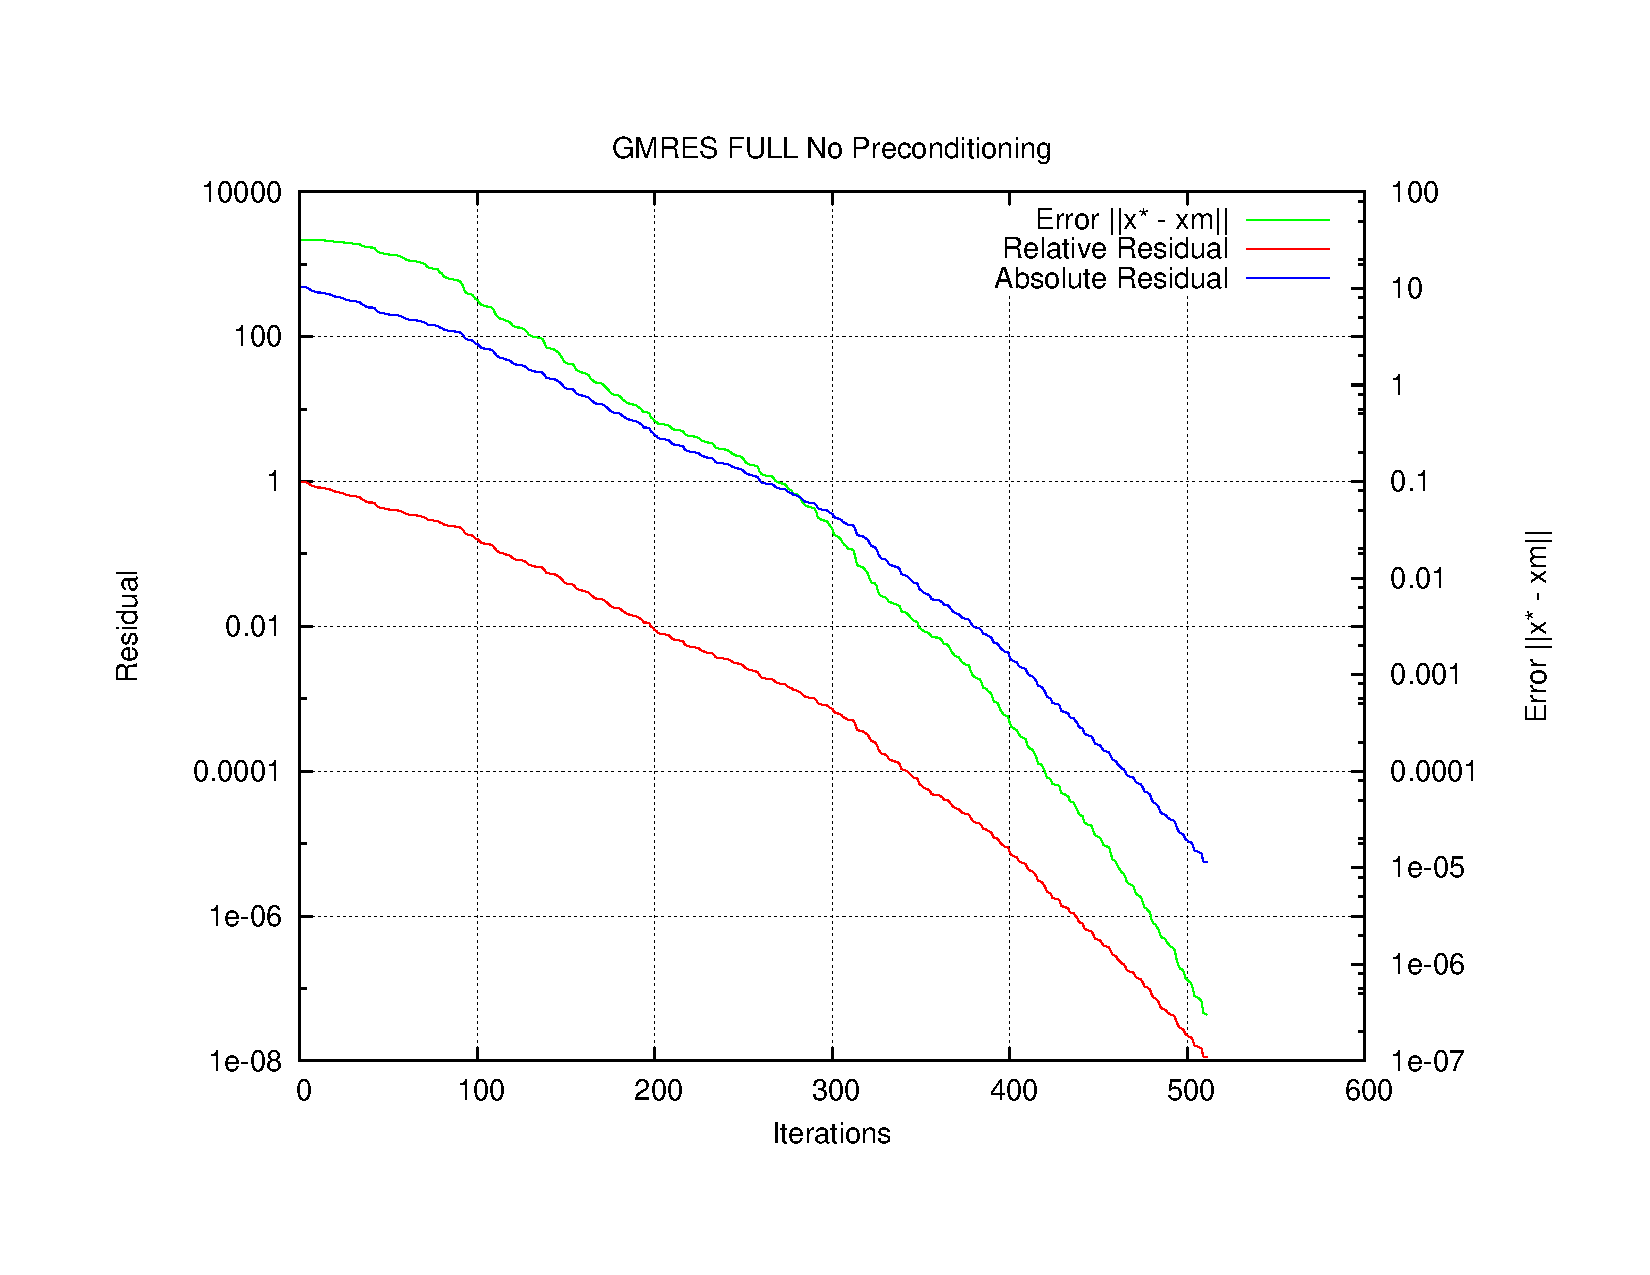
\includegraphics[scale=0.54]{./Output/GMRES_FULL_NO.pdf}\\
\caption{Plot 1: GMRES FULL No Preconditioning}}
\end{center}
\begin{center}
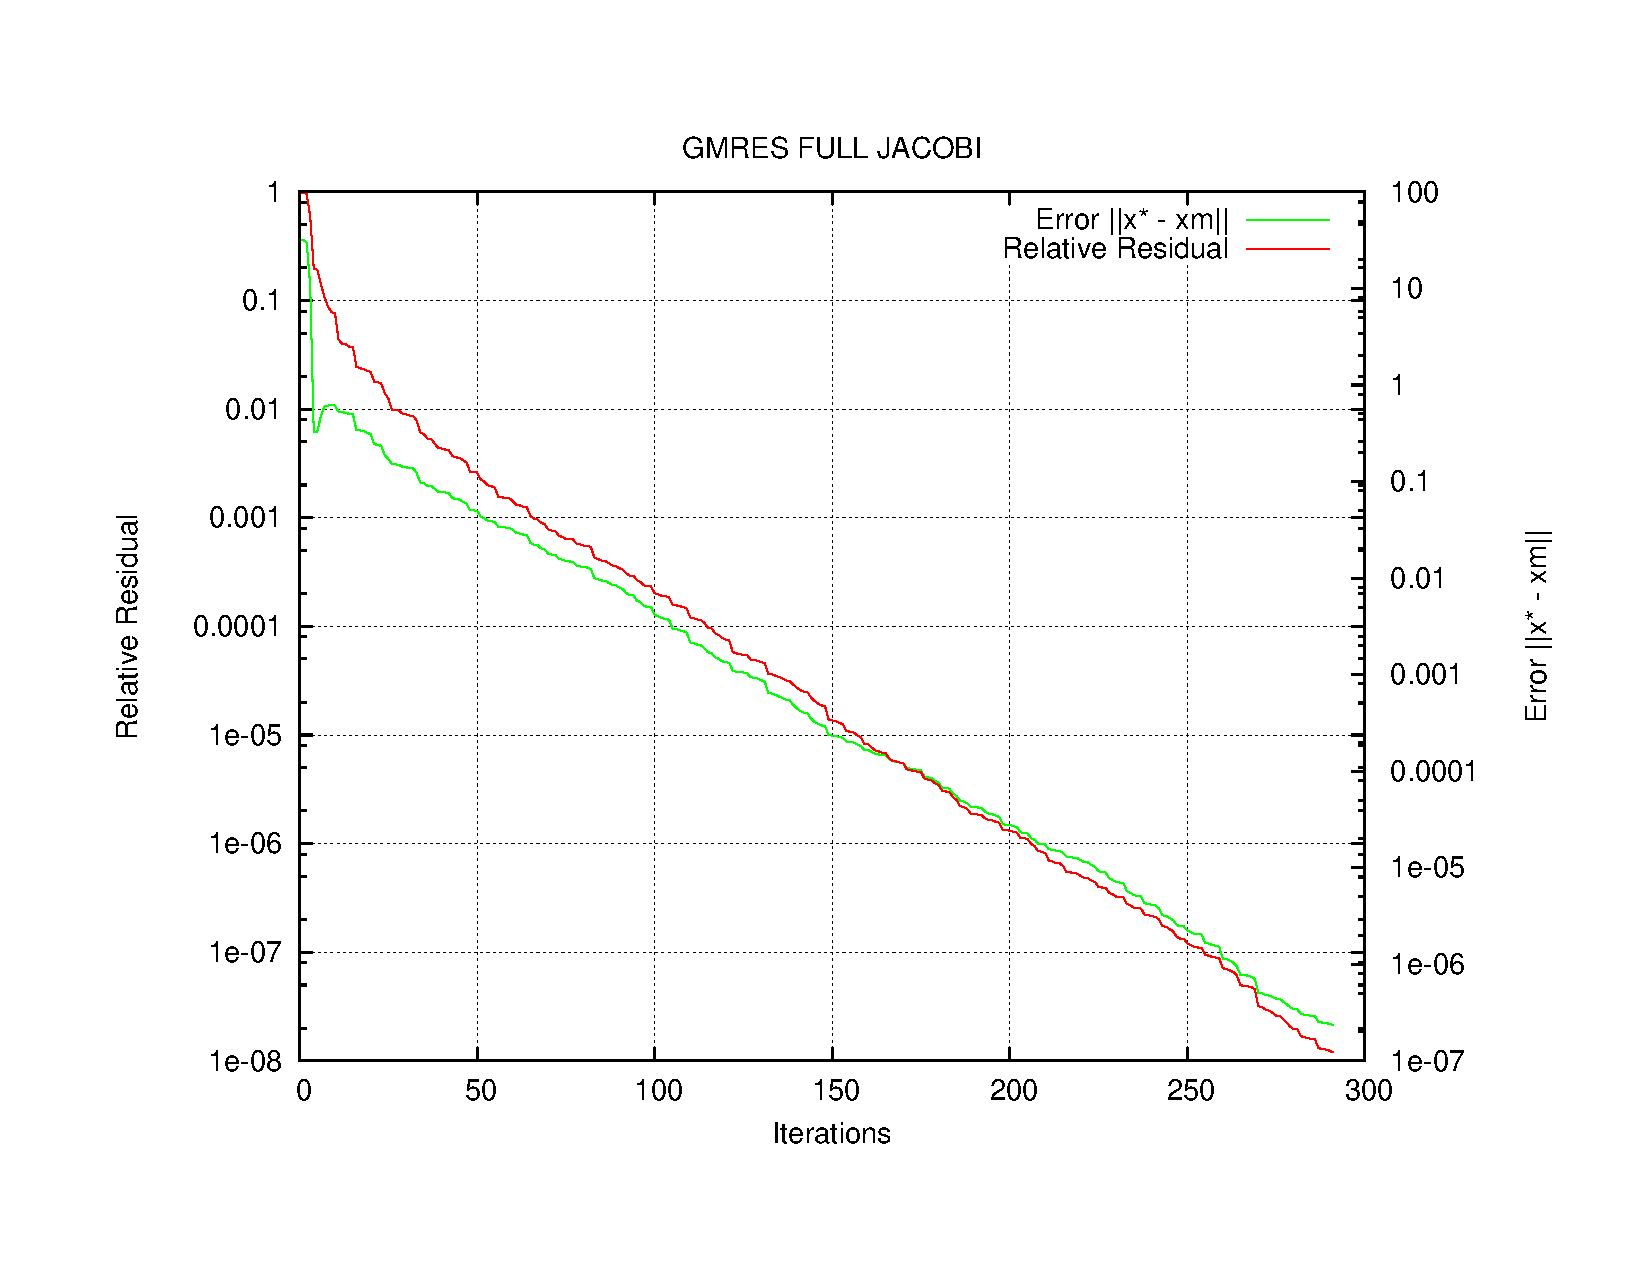
\includegraphics[scale=0.54]{./Output/GMRES_FULL_JACOBI.pdf}\\
\caption{Plot 2: GMRES FULL Jacobi Preconditioning}}
\end{center}
\begin{center}
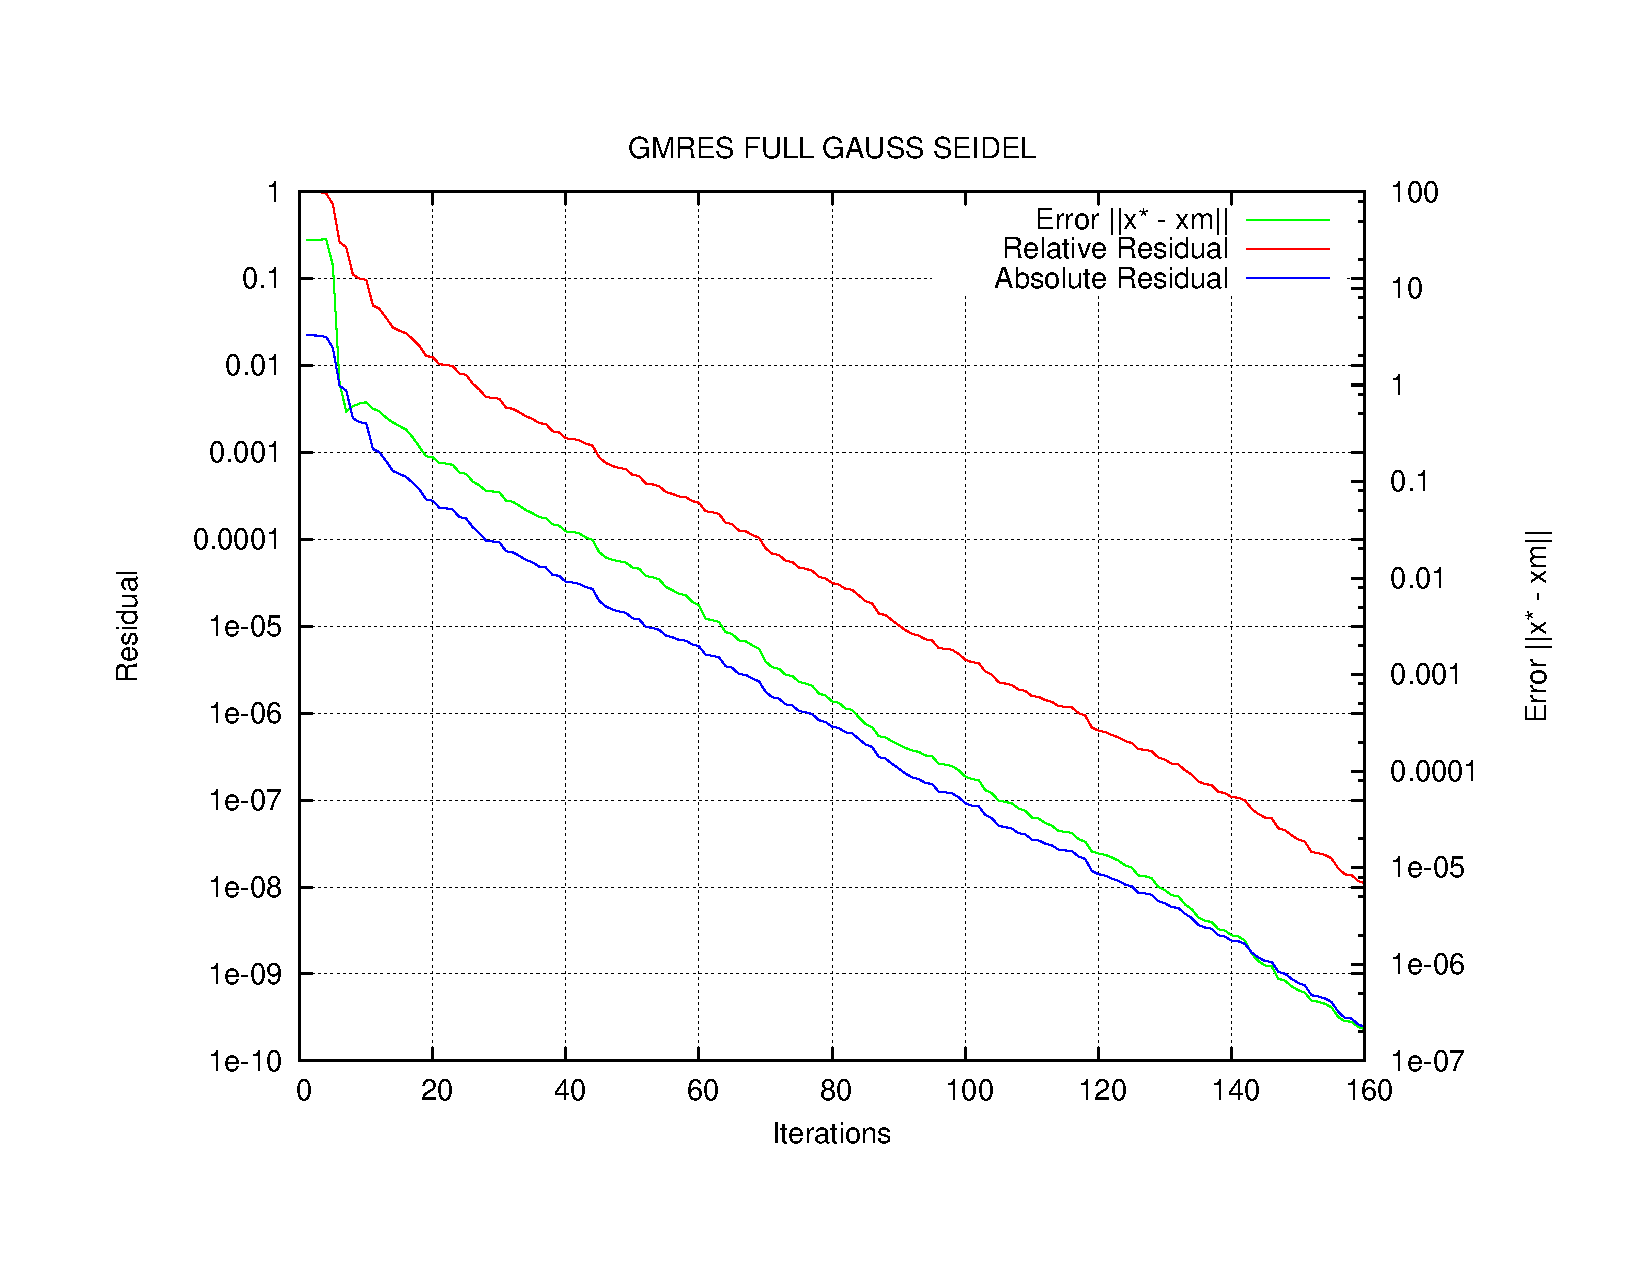
\includegraphics[scale=0.54]{./Output/GMRES_FULL_GAUSS_SEIDEL.pdf}\\
\caption{Plot 3: GMRES FULL Gauss Seidel Preconditioning}}
\end{center}
\begin{center}
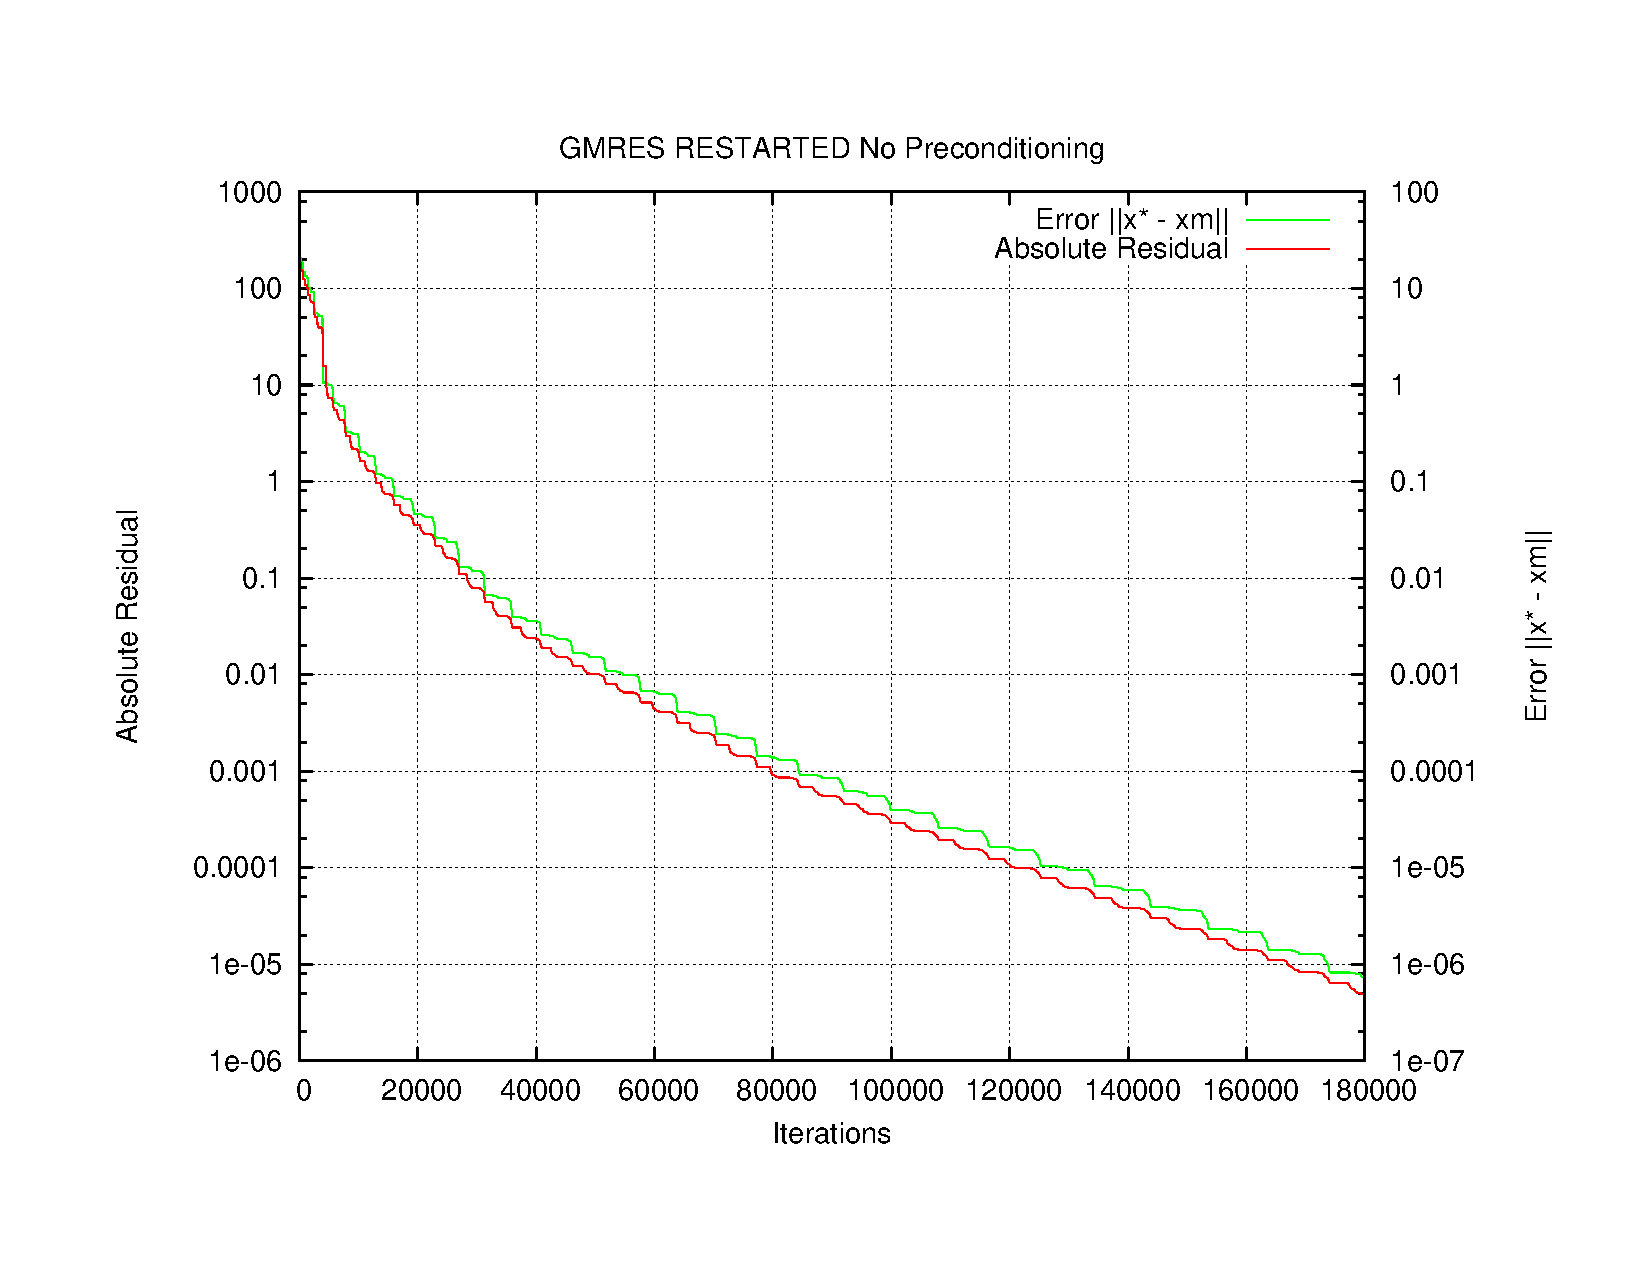
\includegraphics[scale=0.54]{./Output/GMRES_RESTARTED_NO.pdf}\\
\caption{Plot 4: GMRES RESTARTED No Preconditioning}}
\end{center}
\begin{center}
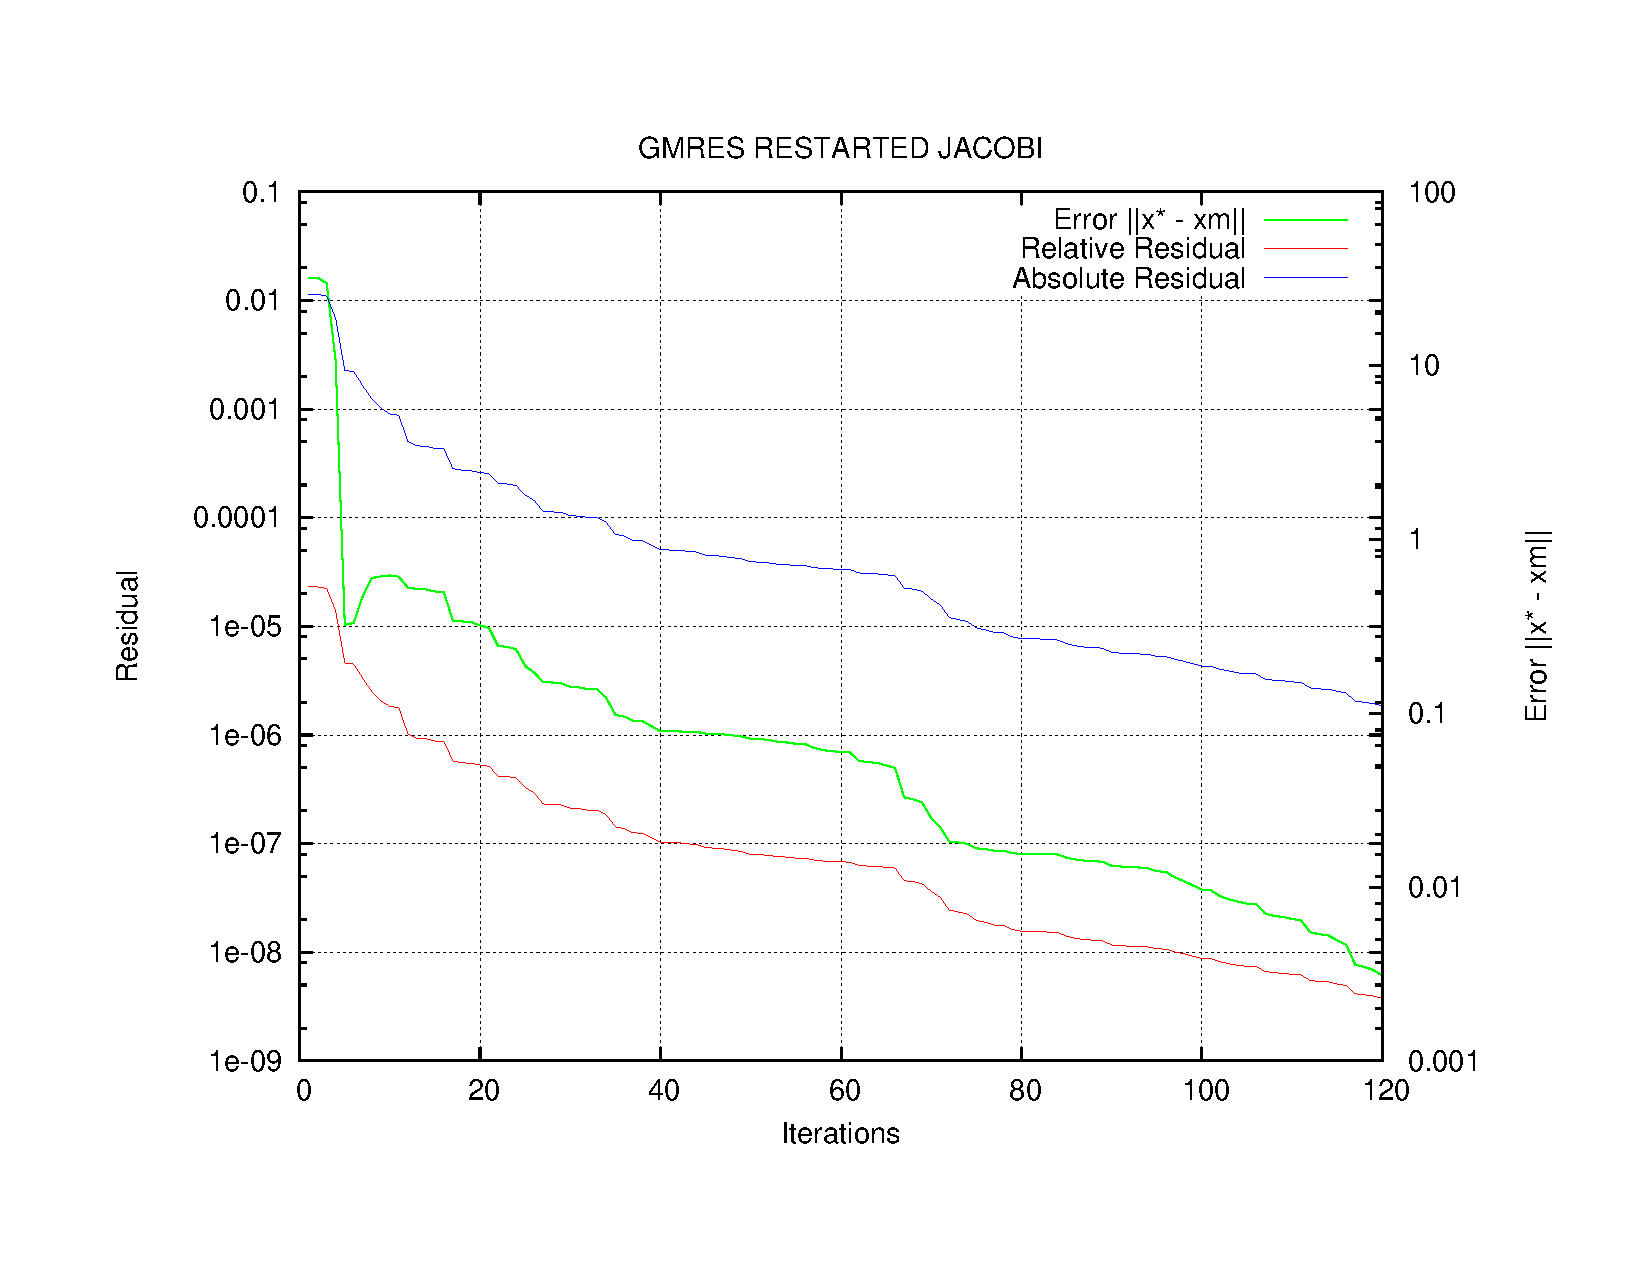
\includegraphics[scale=0.54]{./Output/GMRES_RESTARTED_JACOBI.pdf}\\
\caption{Plot 5: GMRES RESTARTED Jacobi Preconditioning}}
\end{center}
\begin{center}
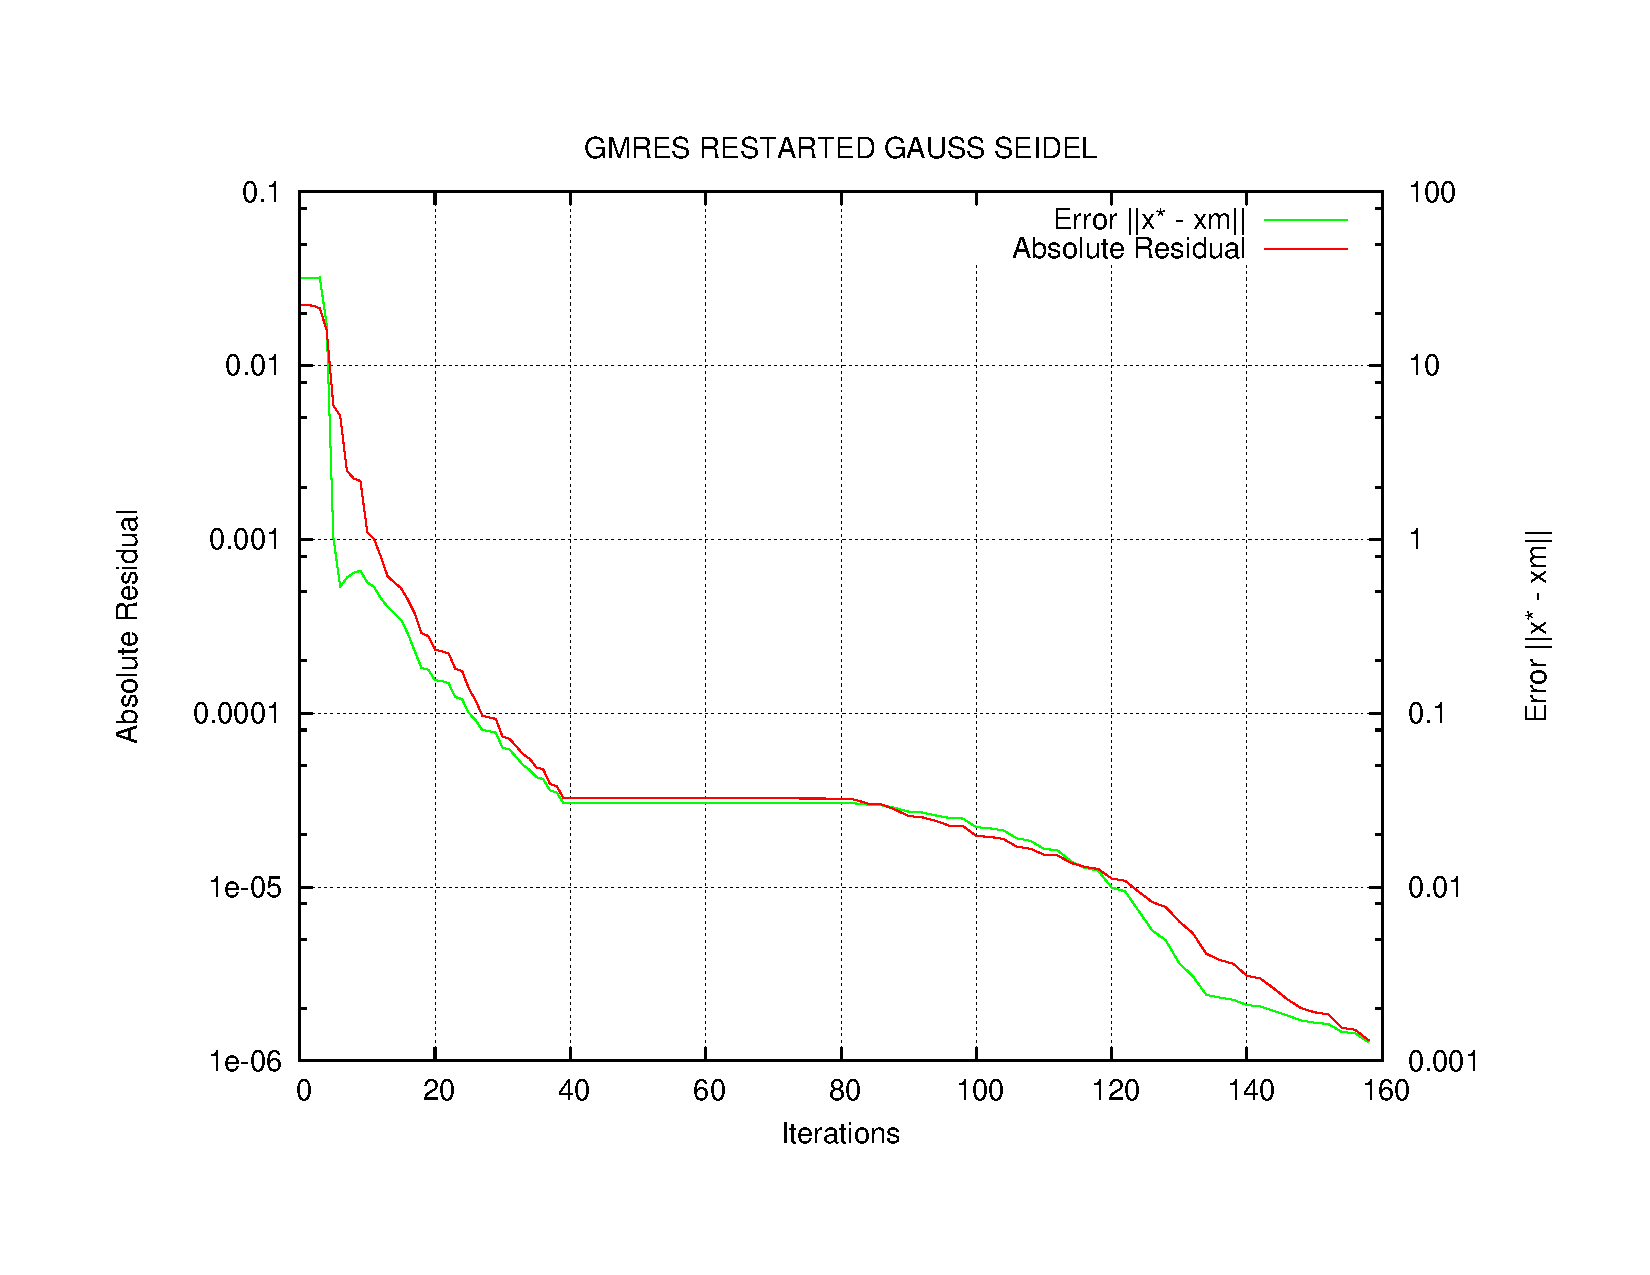
\includegraphics[scale=0.54]{./Output/GMRES_RESTARTED_GAUSS_SEIDEL.pdf}\\
\caption{Plot 6: GMRES RESTARTED Gauss Seidel Preconditioning}}
\end{center}
\begin{center}
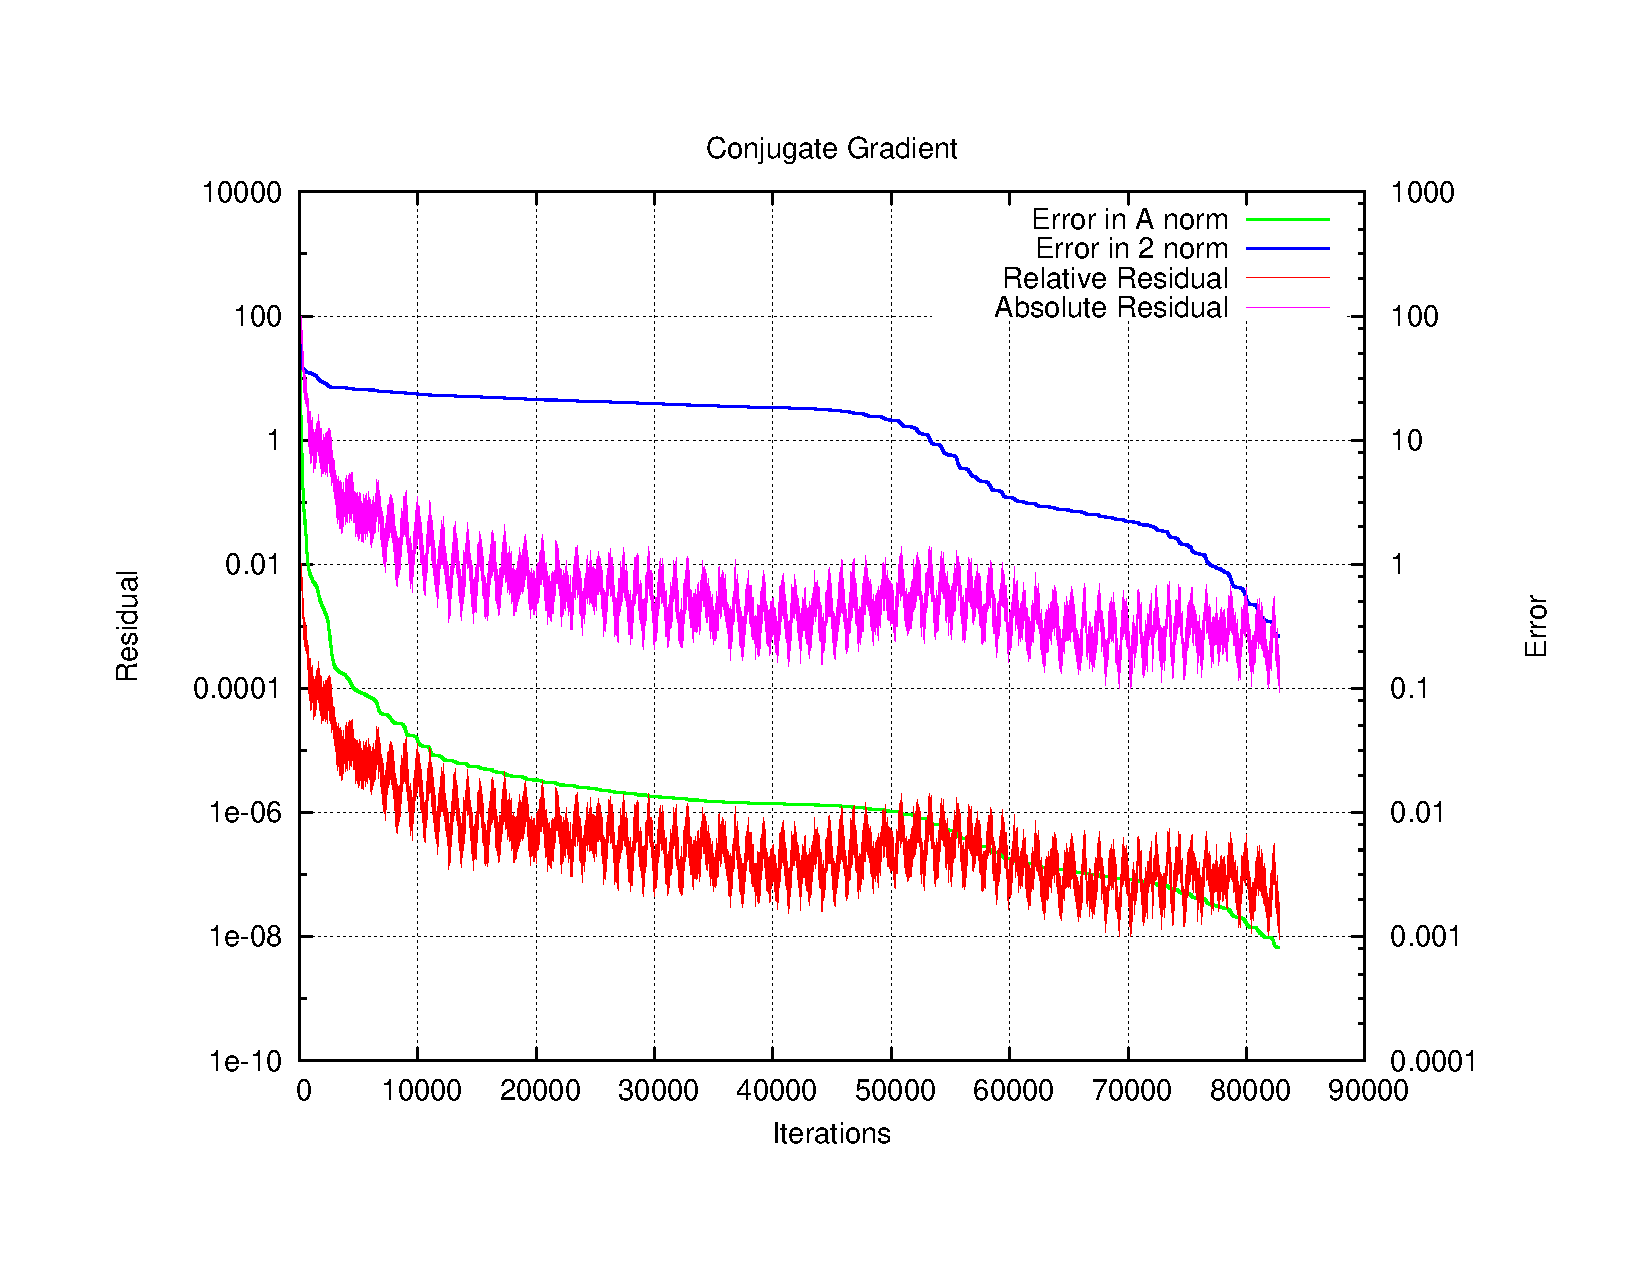
\includegraphics[scale=0.54]{./Output/CG.pdf}\\
\caption{Plot 7: Conjugate Gradient}}
\end{center}
\section{Full GMRES Method:}
1. Without preconditioning, Number of Krylov Vectors required: \textbf{512}\\
2. With Jacobi preconditioning, Number of Krylov Vectors required: \textbf{293}\\
3. With Gauss Seidl preconditioning, Number of Krylov Vectors required: \textbf{161}

\section{Restarted GMRES Method:}
Best restart parameter (m) = 40 with time \sim 0.26-0.28 s.
\\

This is sensitive to the calculation of solution vector within inner for loop that is required to be done in this project to calculated error per iteration. If we calculate 	solution vector at the end instead of calculating it in every iteration, we get best restart parameter as 63. But with the inclusion of calculation of solution vector inside inner for loop offsets the advantage in time that we would have got with 63 krylov vectors.
\\

This optimal method is faster than full GMRES method because the number of Krylov vectors is fixed to a lower number (40) than that required by full GMRES (512) which reduces the number of operations significantly. We are getting 512 Krylov vectors for Full GMRES without preconditioning. With restarted GMRES, m =40 is the best restart parameter and we get 2747 cumulative iterations(\sim 70 	iterations). So, the order of operations is O(70\times 40^2 	). Order of operations in full GMRES is O(512^2 	).
So, we expect the speed up of 70*40*40/512/512 \approx 2.3.

From Plot 8. We can see this.
\\

Additionally, the initial guess is improved at every execution of GMRES algorithm.
\section{Preconditioned GMRES Method:}
\begin{center}
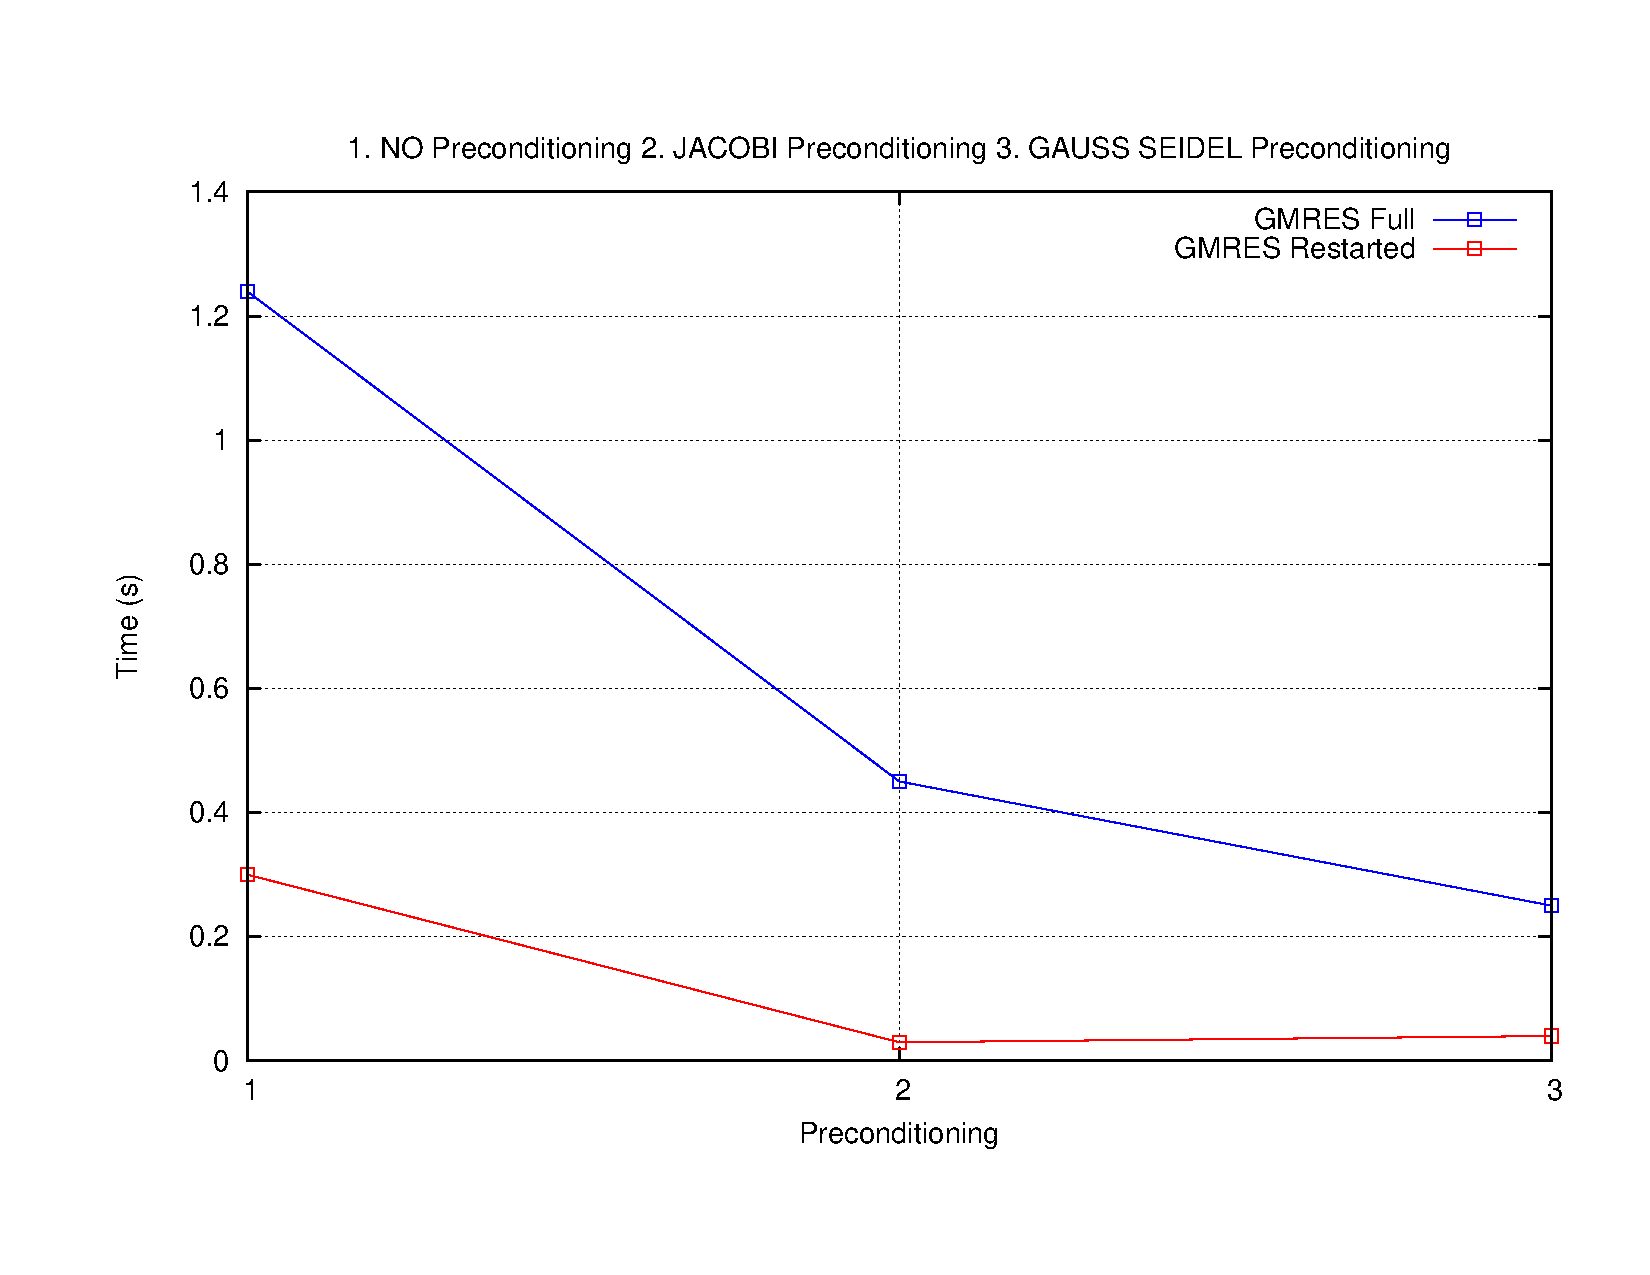
\includegraphics[scale=0.54]{./Output/Timings_GMRES.pdf}\\
\caption{Plot 8: Comparison of Timings with and without preconditioning}}
\end{center}
GMRES Method with Gauss Seidel preconditioning is the fastest one.
\\
As we can see from Plot 9, relative residual that is calculated based on true absolute residual instead of preconditioned residual, stops iterating much before which results in bad error(approx.  0.01). In fact, with preconditioning we are solving system with modified residual, so it makes sense to monitor the modified residual.
\begin{center}
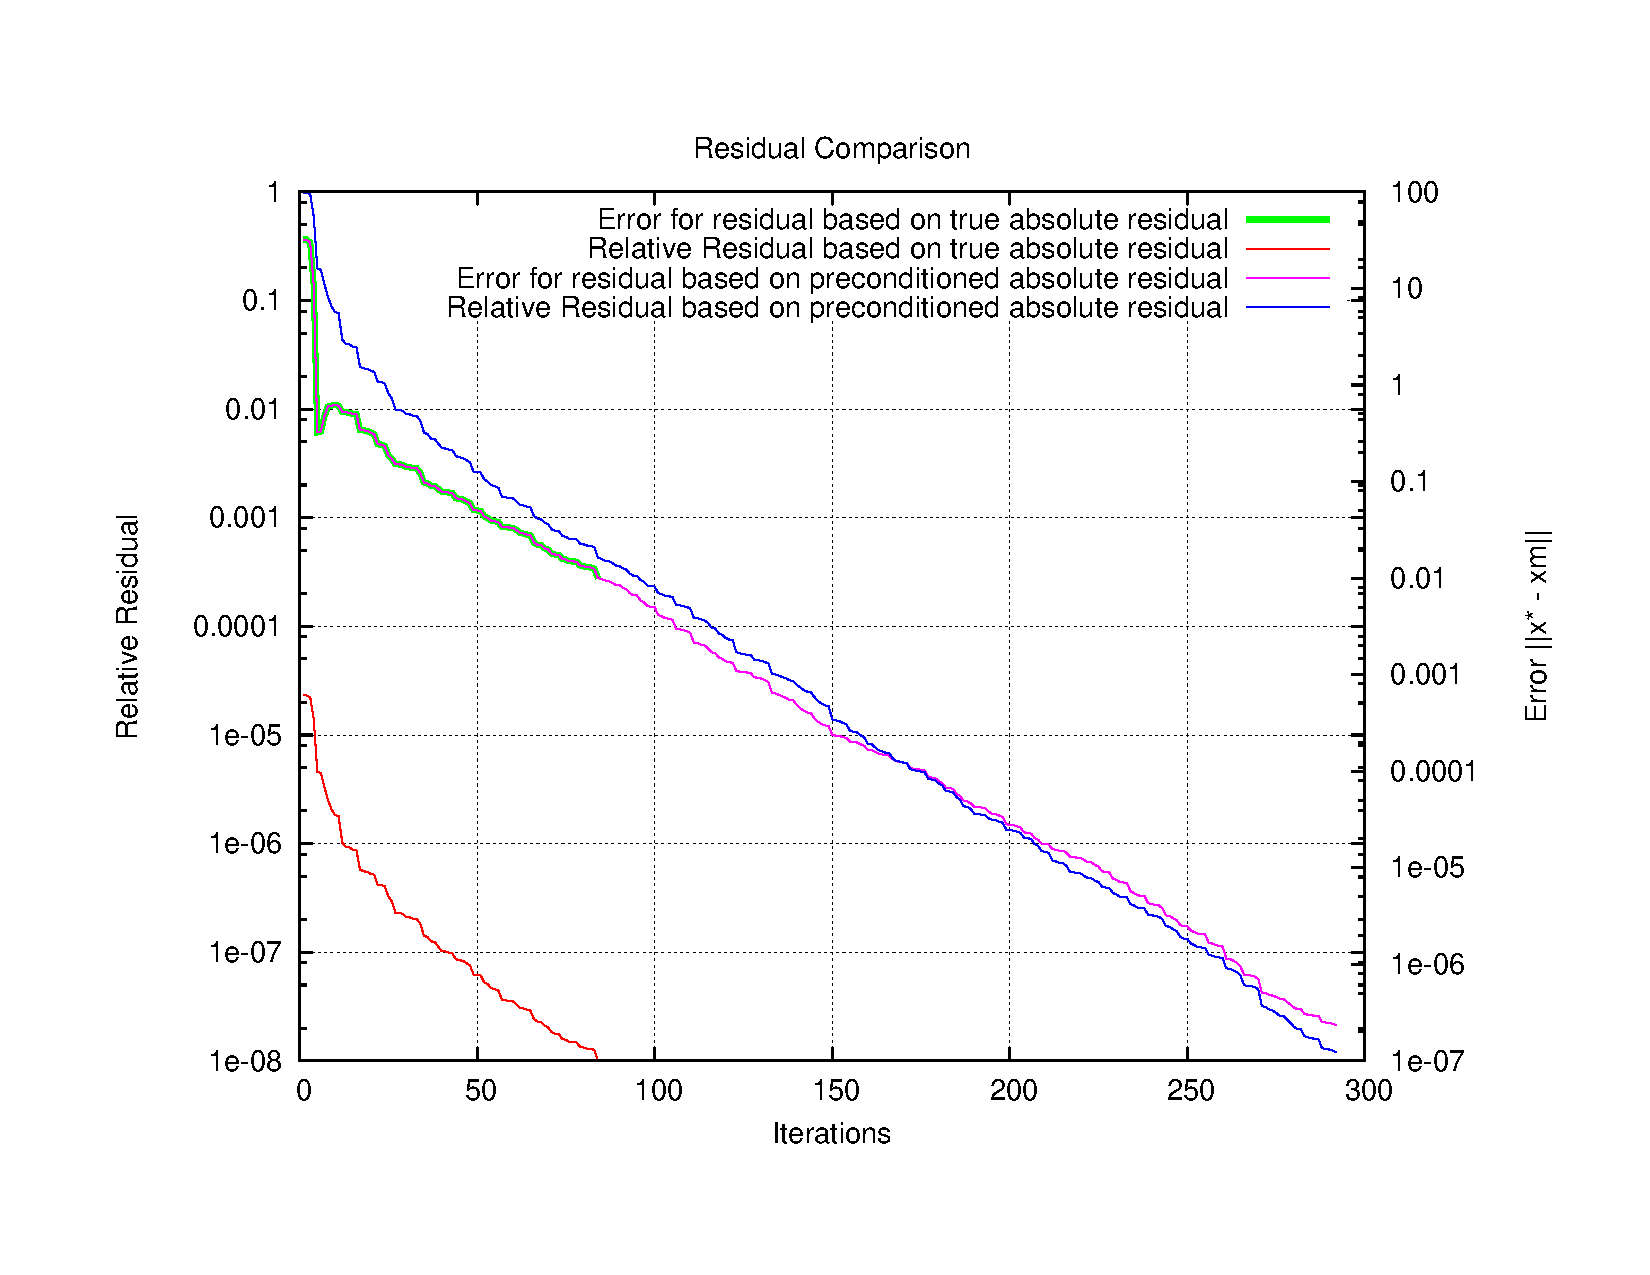
\includegraphics[scale=0.6]{./Output/PRECOND_RES.pdf}\\
\caption{Plot 9: Comparison of Relative Residual based on True and Preconditioned Absolute Residual}}
\end{center}


\section{Conjugate Gradient Method:}
Both the errors, i.e. error in A norm and error in 2 norm are plotted in Plot 7.
\\
By formulation of Conjugate method, we are minimizing error in A-norm. So, we observe monotonic decrease in the error in A-norm. The residual, on the other hand, is oscillating but overall trend is decreasing.

\end{document}